\subsection{Biological testing\label{sec:bio2}}

The biological testing presented in this section was planned by me but carried out by Tom O'Brien, a PhD student in the Department of Biochemistry.

The HSL analogue-ciprofloxacin conjugates (see \ref{fgr:finals_2}), as well as C$_4$-HSL \compound{cmpd:HL4}, ciprofloxacin \compound{cmpd:Cip}, methyl ciprofloxacin \compound{cmpd:CipMe}, the alkynyl ciprofloxacin derivative \compound{cmpd:Y4Cip}, the \textit{tert}-butyl ester methyl ciprofloxacin derivative \compound{cmpd:tBuOO4CipMe} and the carboxylic acid methyl ciprofloxacin derivative \compound{cmpd:HOO4CipMeTFA} were tested for antibacterial and anti-biofilm activity in \textit{P. aeruginosa} PAO1\cite{Stover2000} and YM64\cite{Morita2001}.

\begin{figure}[H]
	\begin{center}
		\schemeref[SHL4CipMe]{cmpd:SHL4CipMe}
		\schemeref[SHL4T4Cip]{cmpd:SHL4T4Cip}
		\schemeref[SHL4THCip]{cmpd:SHL4THCip}
		\schemeref[SHL4TMeCip]{cmpd:SHL4TMeCip}
		\schemeref[2MeOA4CipMe]{cmpd:2MeOA4CipMe}
		\schemeref[3MeOA4CipMe]{cmpd:3MeOA4CipMe}
		\schemeref[2MeOA4T4Cip]{cmpd:2MeOA4T4Cip}
		\schemeref[3MeOA4T4Cip]{cmpd:3MeOA4T4Cip}
		\schemeref[HOcy5NH4CipMe_RR]{cmpd:HOcy5NH4CipMe_RR}
		\schemeref[HOcy5NH4CipMe_SS]{cmpd:HOcy5NH4CipMe_SS}
		\schemeref[Ocy5NH4CipMe_S]{cmpd:Ocy5NH4CipMe_S}
		\schemeref[HOcy5NH4T4Cip_RR]{cmpd:HOcy5NH4T4Cip_RR}
		\schemeref[HOcy5NH4T4Cip_SS]{cmpd:HOcy5NH4T4Cip_SS}
		\schemeref[HOcy6NH4CipMe]{cmpd:HOcy6NH4CipMe}
		\schemeref[Ocy6NH4CipMe]{cmpd:Ocy6NH4CipMe}
		\schemeref[HOcy6NH4T4Cip]{cmpd:HOcy6NH4T4Cip}
		\schemeref[Ocy6NH4T4Cip]{cmpd:Ocy6NH4T4Cip}
		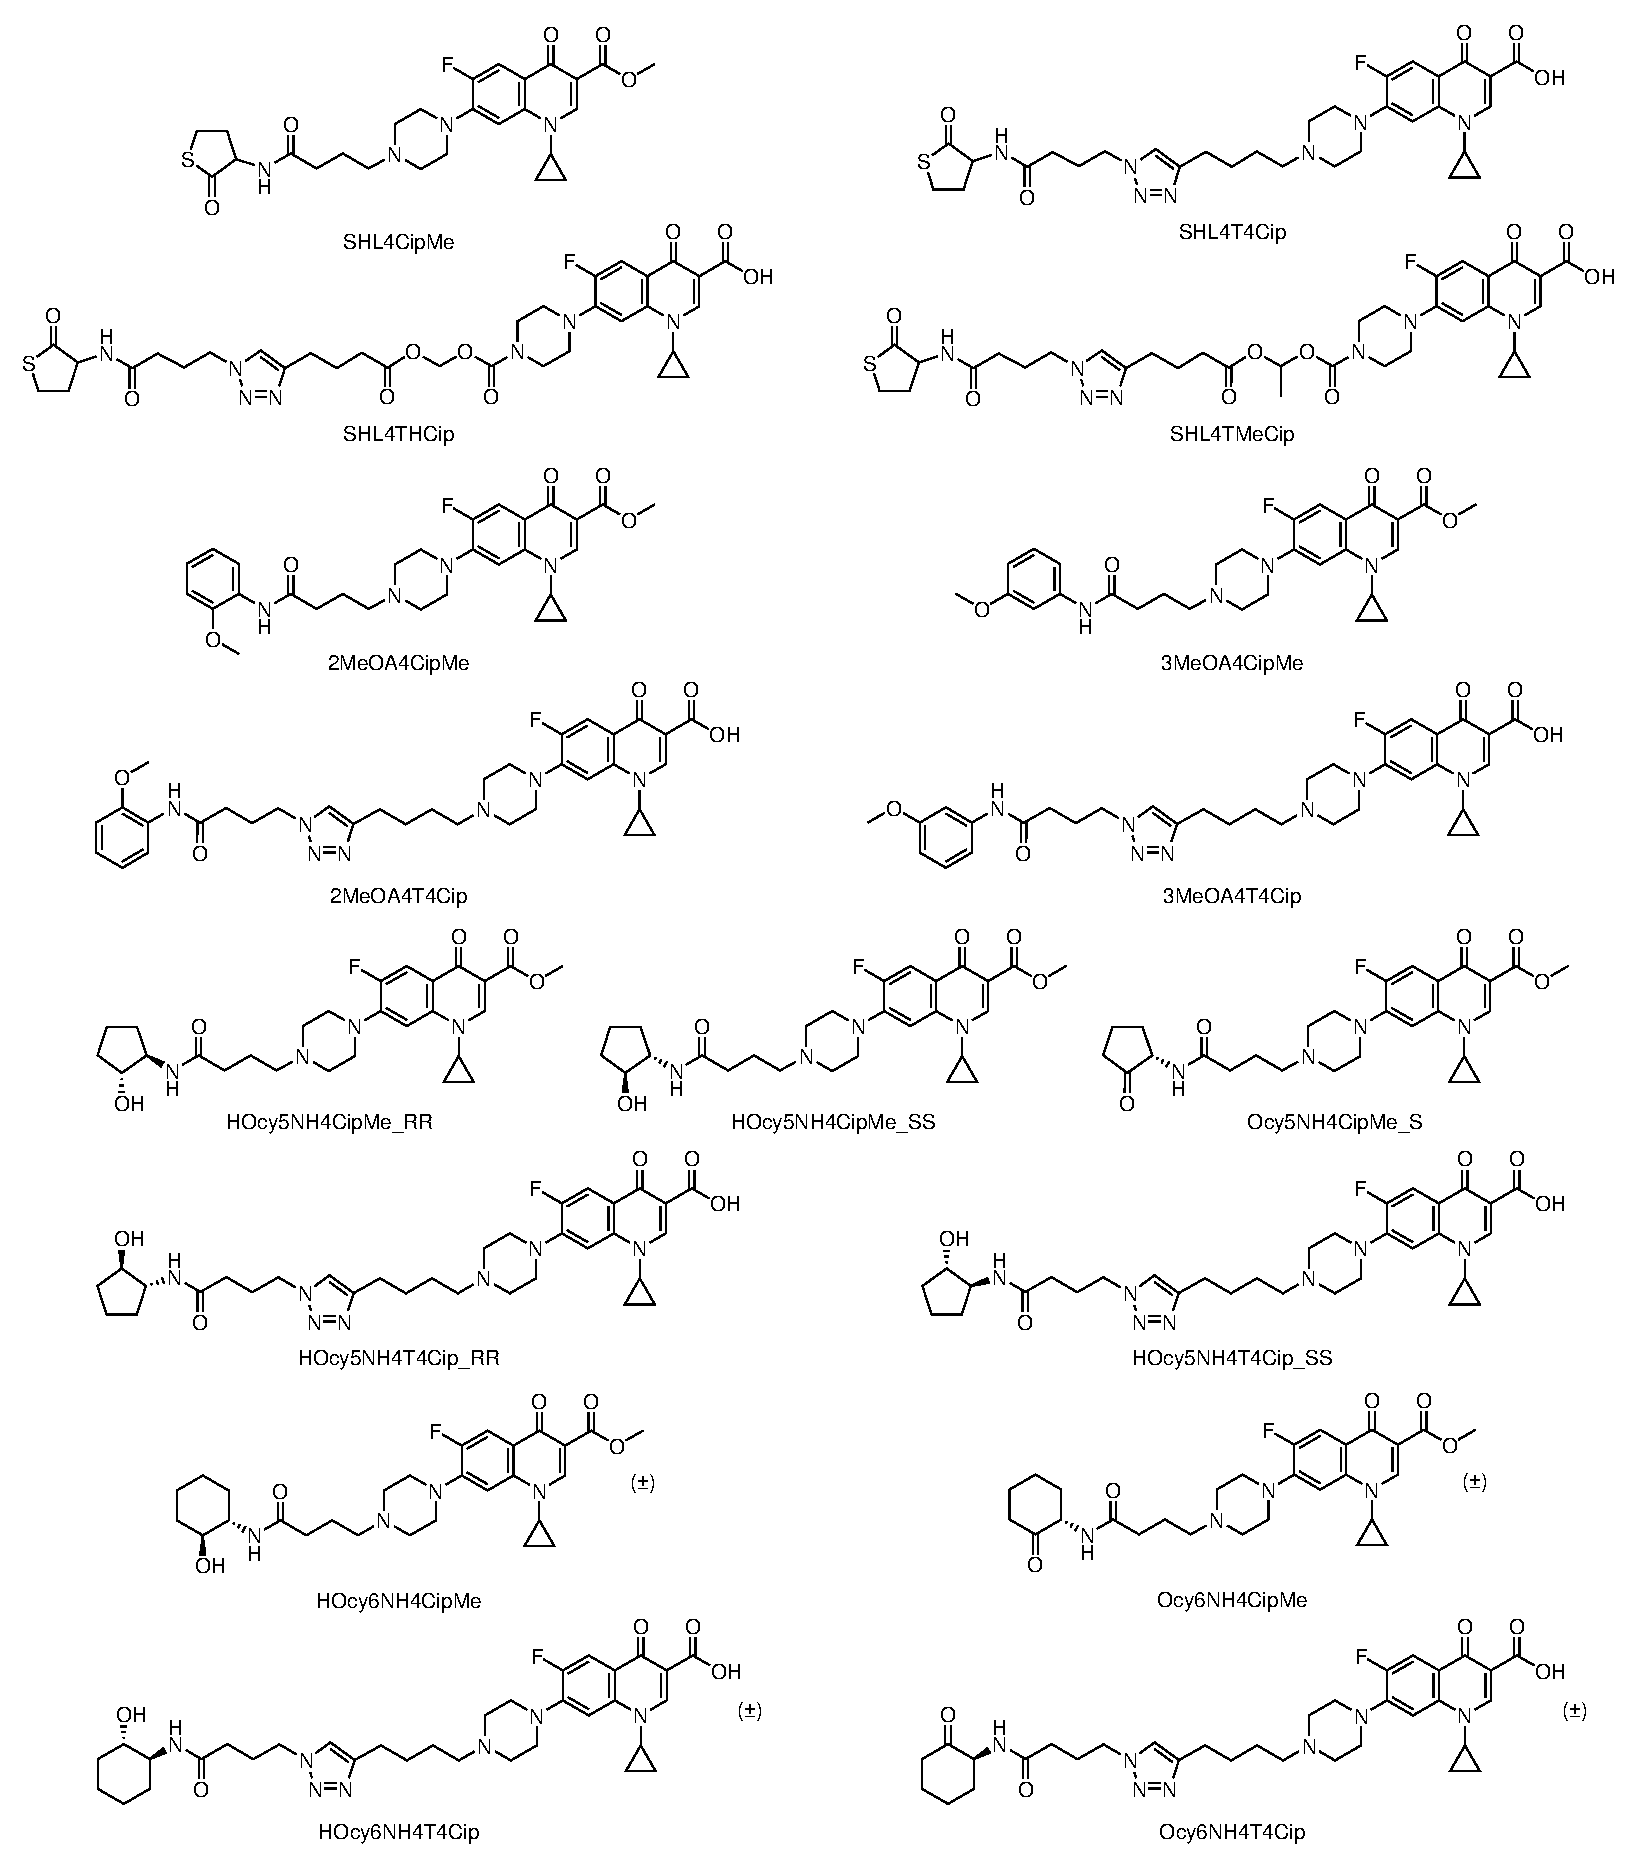
\includegraphics[scale=0.5]{finals_2}
		\caption{The HSL analogue-ciprofloxacin conjugates.
 		\label{fgr:finals_2}}
	\end{center}
\end{figure}

\subsubsection{Antibacterial activity}

%The Minimum Inhibitory Concentration (MIC) is defined as the lowest concentration of an antimicrobial ingredient or agent that is bacteriostatic (prevents the visible growth of bacteria). MICs are used to evaluate the antimicrobial efficacy of various compounds by measuring the effect of decreasing concentrations of antibiotic/antiseptic over a defined period in terms of inhibition of microbial population growth.  

\subsubsubsection{YM64}

In YM64 at 5 h several of the HSL analogue-ciprofloxacin conjugates showed activity at the highest concentration (see \ref{fgr:YM64_5h_S} and \ref{fgr:YM64_5h_HO}). 
Conjugates \compound{cmpd:2MeOA4T4Cip} and \compound{cmpd:3MeOA4T4Cip} showed similar activity to ciprofloxacin \compound{cmpd:Cip} and the cleavable conjugate
\compound{cmpd:SHL4THCip} showed better activity (see \ref{fgr:YM64_5h_S}).
The activity of the cleavable conjugate \compound{cmpd:SHL4THCip} was even more pronounced at 24 h (see \ref{fgr:YM64_24h_S}).

It should be noted that the highest concentration tested was 25 $\mu$M in this set of assays as opposed to 2 $\mu$M in the previous set (see \ref{sec:bio1}), but oddly all compounds including ciprofloxacin \compound{cmpd:Cip} showed less activity. This is thought to be due to a change in the plate seals used and/or the humidity of the incubation conditions (see \ref{sec:exp_bio}). 

%trim=left bottom right top

\begin{figure}[H]
	\begin{center}
		\includegraphics[width=\textwidth,trim={1cm 1cm 1cm 1cm},clip]{"Biochem - YM64_5h_S"}
		\caption{YM64 OD readings at 5 h for the HCTL, 2-methoxybenzene and 3-methoxybenzene HSL analogue-ciprofloxacin conjugates.\label{fgr:YM64_5h_S}}
	\end{center}
\end{figure}

\begin{figure}[H]
	\begin{center}
		\includegraphics[width=\textwidth,trim={1cm 1cm 1cm 1cm},clip]{"Biochem - YM64_5h_HO"}
		\caption{YM64 OD readings at 5 h for the alcohol and ketone HSL analogue-ciprofloxacin conjugates.\label{fgr:YM64_5h_HO}}
	\end{center}
\end{figure}

\begin{figure}[H]
	\begin{center}
		\includegraphics[width=\textwidth,trim={1cm 1cm 1cm 1cm},clip]{"Biochem - YM64_24h_S"}
		\caption{YM64 OD readings at 24 h for the HCTL, 2-methoxybenzene and 3-methoxybenzene HSL analogue-ciprofloxacin conjugates.\label{fgr:YM64_24h_S}}
	\end{center}
\end{figure}

\begin{figure}[H]
	\begin{center}
		\includegraphics[width=\textwidth,trim={1cm 1cm 1cm 1cm},clip]{"Biochem - YM64_24h_HO"}
		\caption{YM64 OD readings at 24 h for the alcohol and ketone HSL analogue-ciprofloxacin conjugates.\label{fgr:YM64_24h_HO}}
	\end{center}
\end{figure}

%Growth curves for interesting ones at lowest conc compare to controls?
%9,10,11,12,15,16
%17-21,24,25
%Best 10,11,12,15,16,20,21,24,25

\subsubsubsection{PAO1}

In PAO1 at 5 h conjugates \compound{cmpd:SHL4THCip}, \compound{cmpd:2MeOA4T4Cip} and \compound{cmpd:3MeOA4T4Cip} showed activity at the highest concentration (see \ref{fgr:PAO1_5h_S}). 
The cleavable conjugate \compound{cmpd:SHL4THCip} showed similar activity to ciprofloxacin \compound{cmpd:Cip}.
At 24 h conjugate \compound{cmpd:3MeOA4T4Cip} still showed some activity, and
cleavable conjugate \compound{cmpd:SHL4THCip} showed similar activity to ciprofloxacin \compound{cmpd:Cip} (see \ref{fgr:PAO1_24h_S}).


%10,11,12,15,16,20,21,24,25 (13,14 weird)


\begin{figure}[H]
	\begin{center}
		\includegraphics[width=\textwidth,trim={1cm 1cm 1cm 1cm},clip]{"Biochem - PAO1_5h_S"}
		\caption{PAO1 OD readings at 5 h for the HCTL, 2-methoxybenzene and 3-methoxybenzene HSL analogue-ciprofloxacin conjugates.\label{fgr:PAO1_5h_S}}
	\end{center}
\end{figure}

\begin{figure}[H]
	\begin{center}
		\includegraphics[width=\textwidth,trim={1cm 1cm 1cm 1cm},clip]{"Biochem - PAO1_5h_HO"}
		\caption{PAO1 OD readings at 5 h for the alcohol and ketone HSL analogue-ciprofloxacin conjugates.\label{fgr:PAO1_5h_HO}}
	\end{center}
\end{figure}


\begin{figure}[H]
	\begin{center}
		\includegraphics[width=\textwidth,trim={1cm 1cm 1cm 1cm},clip]{"Biochem - PAO1_24h_S"}
		\caption{PAO1 OD readings at 24 h for the HCTL, 2-methoxybenzene and 3-methoxybenzene HSL analogue-ciprofloxacin conjugates.\label{fgr:PAO1_24h_S}}
	\end{center}
\end{figure}

\begin{figure}[H]
	\begin{center}
		\includegraphics[width=\textwidth,trim={1cm 1cm 1cm 1cm},clip]{"Biochem - PAO1_24h_HO"}
		\caption{PAO1 OD readings at 24 h for the alcohol and ketone HSL analogue-ciprofloxacin conjugates.\label{fgr:PAO1_24h_HO}}
	\end{center}
\end{figure}

%
%
%
%
%Approximate MICs for the more active compounds are shown in \ref{tbl:MICs}
%
%\begin{table}[H]
%  \centering
%\begin{tabular}{|p{0.12\textwidth}|p{0.08\textwidth}|p{0.08\textwidth}|p{0.08\textwidth}|p{0.08\textwidth}|}
%\hline  
%\textbf{Compound} & \textbf{YM64 - 5 h} & \textbf{YM64 - 24 h} & \textbf{PAO1 - 5 h} & \textbf{PAO1 - 24 h} \\ 
%\hline 
%SHL4THCip \compound{cmpd:SHL4THCip} &  &  &  & 0.0455 $\pm$ \\ 
%\hline 
%2MeOA4T4Cip \compound{cmpd:2MeOA4T4Cip} & 0.0406 $\pm$ & 0.0391 $\pm$ &  &  \\ 
%\hline 
%3MeOA4T4Cip \compound{cmpd:3MeOA4T4Cip} &  & 0.0364 $\pm$ &  &  \\ 
%\hline 
%Cip \compound{cmpd:Cip} &  &  &  &  \\ 
%\hline
%\end{tabular}
%\caption{.\label{tbl:}} 
%\end{table}

In addition to its promising antibacterial activity, the cleavable HCTL-ciprofloxacin triazole conjugate \compound{cmpd:SHL4THCip} has an interesting growth curve (see \ref{fgr:growth}).
When \textit{P. aeruginosa} PAO1 is treated with 25 $\mu$M ciprofloxacin \compound{cmpd:Cip} it continues to grow slowly over the course of a 48 h assay, whereas growth is fully inhibited by treatment with the HCTL-ciprofloxacin triazole conjugate \compound{cmpd:SHL4THCip}. However, the errors in this data are large and so the assay needs repeating to confirm the effect.

\begin{figure}[H]
	\begin{center}
		\includegraphics[width=\textwidth,trim={1cm 1cm 1cm 1cm},clip]{"Biochem - Growth"}
		\caption{PAO1 25 $\mu$M.\label{fgr:growth}}
	\end{center}
\end{figure}

\subsubsection{Determination of anti-biofilm activity}

Biofilm inhibition and dispersal were measured using crystal violet staining  (see \ref{sec:exp_bio}). Unfortunately the results were largely unreliable as it was obvious that staining was higher in the wells at the edges of the plates, and that this was overwhelming any other trends. This effect was probably due to increased evaporation from the outer wells. 
It is likely that this effect was seen in these results, but not those in \ref{sec:bio1}, due to a change in the conditions that the plates were incubated in. Specifically, a different type of plate seal was used and a humid environment was maintained in the incubator in the previous experiments (see \ref{sec:exp_bio}).